\documentclass{book}
\usepackage{graphicx}
\usepackage[a4paper, landscape]{geometry}
\usepackage{tikz}
\usepackage{pifont}
\usepackage{varwidth}


\begin{document}

\pagestyle{empty}
\pagenumbering{gobble}

\colorlet{MyColor1}{blue!60!green!80}
\colorlet{MyColor2}{yellow!80}
\colorlet{MyColor3}{black}
\colorlet{MyColor4}{red!70!yellow!50!blue!70}

\def\x{4cm}
\def\y{2.5cm}
\def\h{16cm}
\def\w{10cm}
\def\d{1cm}

% Front Cover
\begin{tikzpicture}[remember picture,overlay,shift={(current page.south west)}]

% Front picture
\node[anchor=south west] at (\x-9cm,\y-0.12cm) {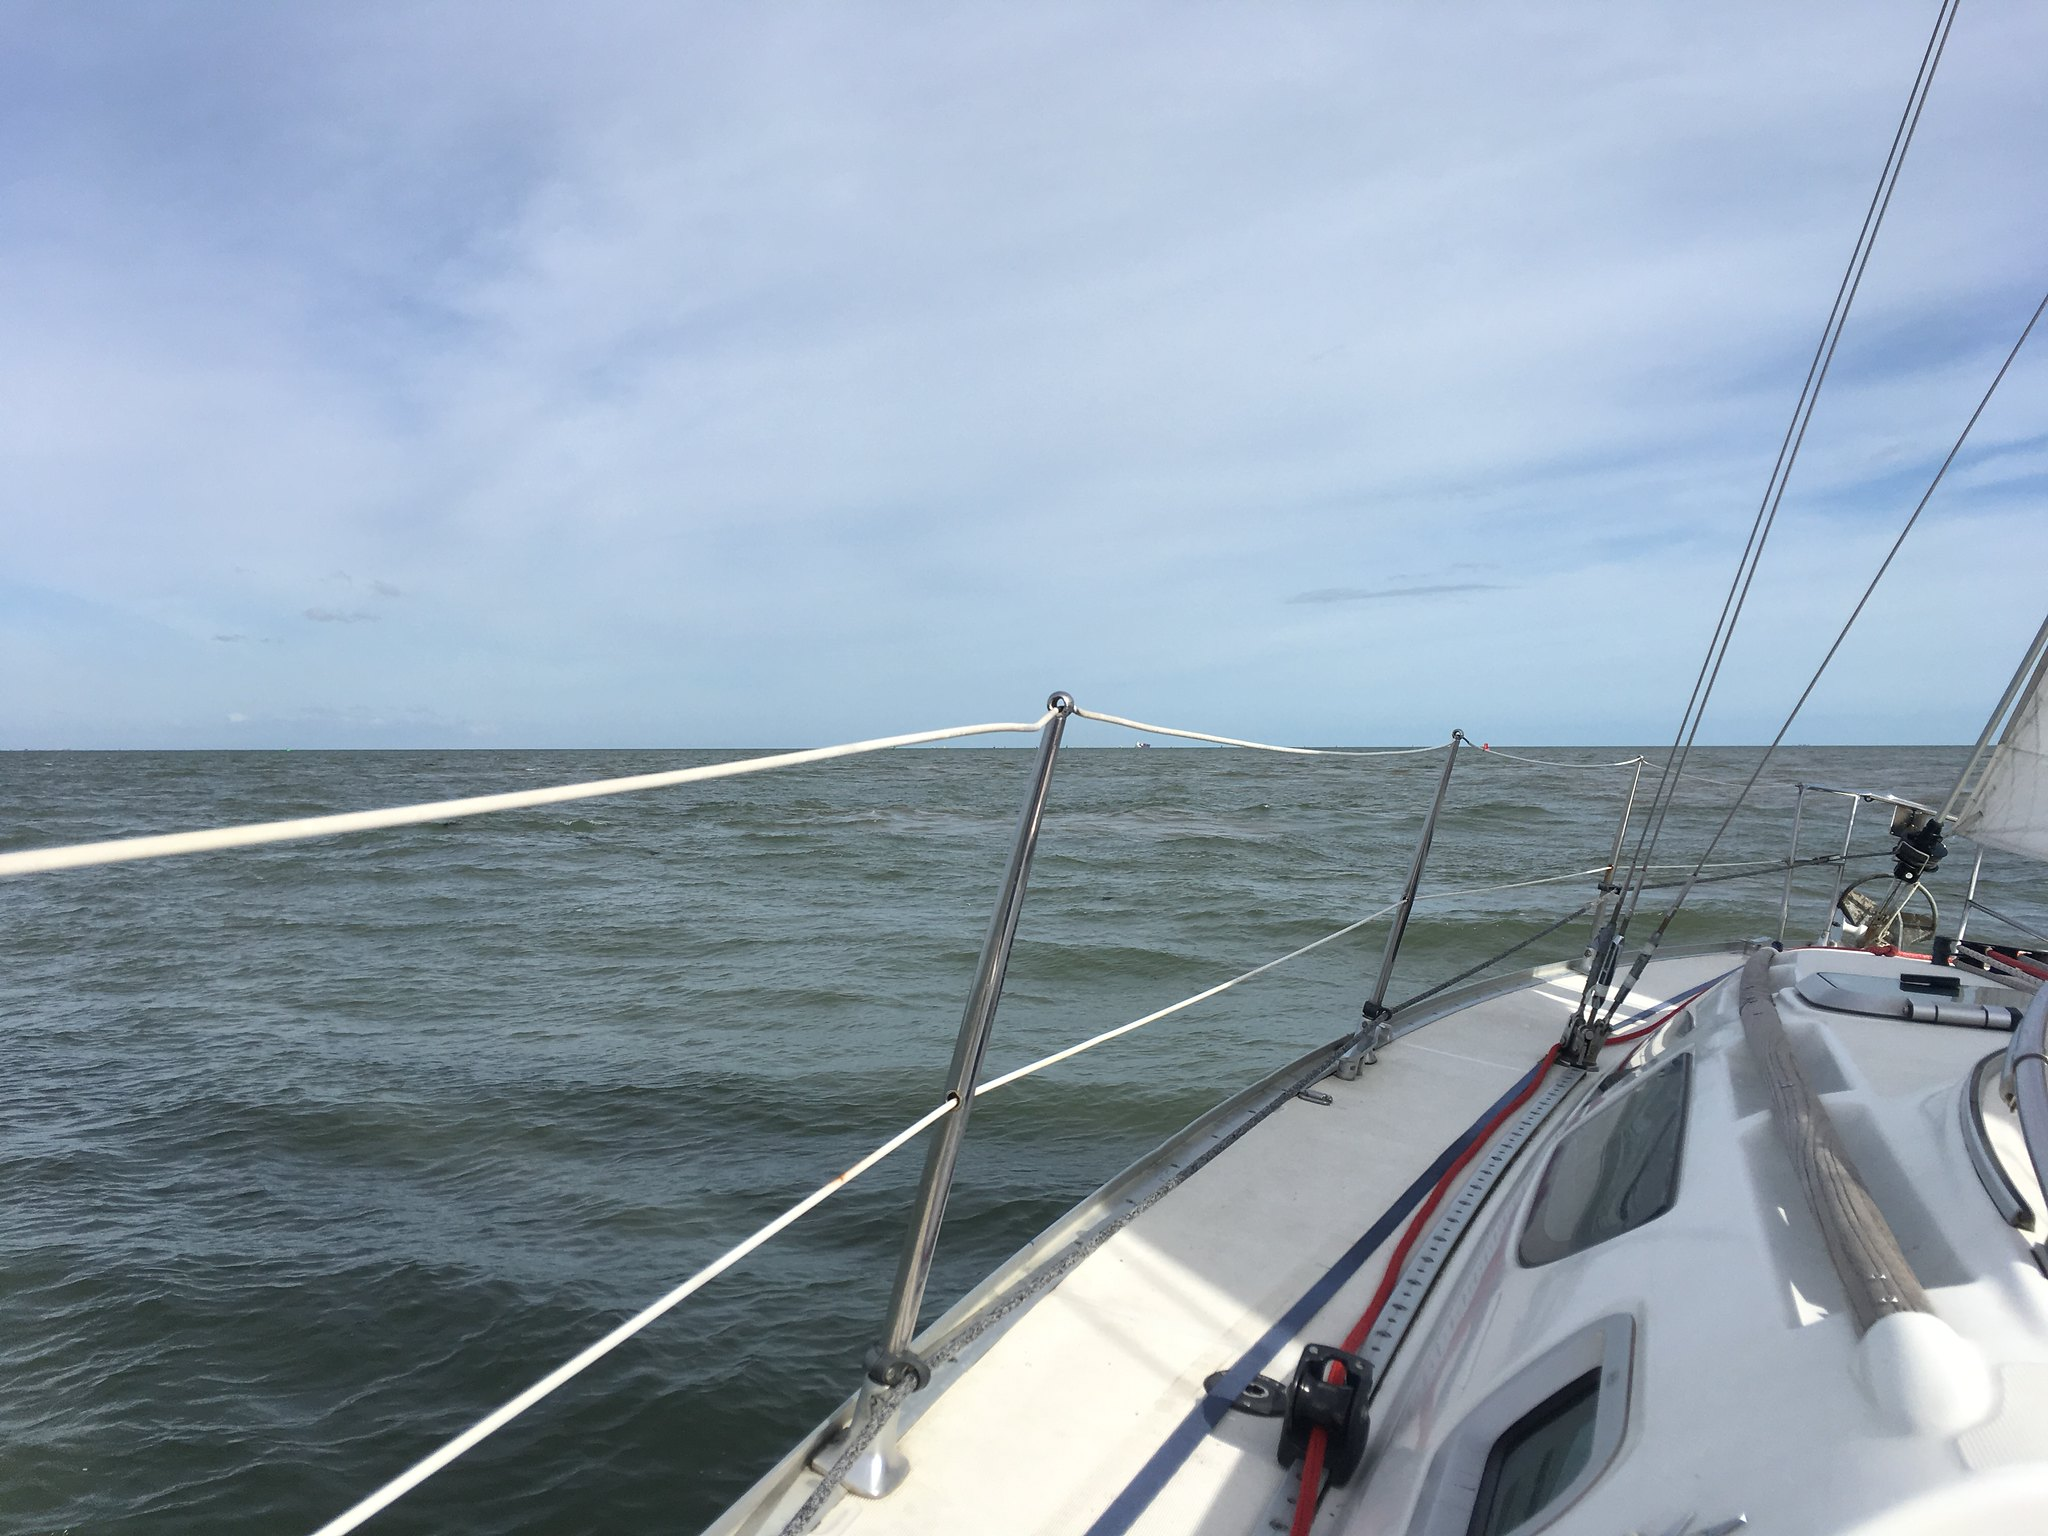
\includegraphics[height=\h]{art/image2}};
% Trim front picture
\draw [fill=white,draw=white] (\x+\w,\y) rectangle +(\d,\h);
\draw [fill=white,draw=white] (0,\y) rectangle +(\x,\h);
% Frame for front picture
\draw [draw=MyColor1,draw=MyColor3] (\x,\y) rectangle +(\w,\h);

% Front title
\begin{Huge}
\begin{bf}
\node[anchor=north west,align=left] at (\x+1cm,\y+\h-2cm) {MY \\ TITLE};
\end{bf}
\end{Huge}

% Front sub-title
\begin{large}
\node[anchor=north west,align=left,text=white!30,] at (\x+2.5cm,\y+7.8cm) {My \\ Sub Title};
\end{large}

\end{tikzpicture}


% Spine
\begin{tikzpicture}[remember picture,overlay,shift={(current page.south west)}]
\draw [fill=MyColor4,draw=MyColor3] (\x+\w,\y) rectangle +(\d,\h);
\node[anchor=center,text=white!30,rotate=90] at (\x+\w+\d/2,\y+8cm) {MY TITLE};
\end{tikzpicture}


% Back Cover
\begin{tikzpicture}[remember picture,overlay,shift={(current page.south west)}]

\draw [draw=MyColor1,fill=MyColor1,draw=MyColor3] (\x+\w+\d,\y) rectangle +(\w,\h);

\begin{large}
\node[anchor=center,align=left,text=MyColor2,text width=7.5cm] at (\x+\w+\d+5cm,\y+8cm) {
\begin{varwidth}{\linewidth}
Back-cover description:
\begin{itemize}
\item [\ding{42}] Item 1
\item [\ding{42}] Item 2
\item [\ding{42}] Item 3
\end{itemize}
\end{varwidth}
};
\end{large}

\end{tikzpicture}

\end{document}
